\chapter{QAOA for Max-Cut}
The aim of Max-Cut is to find a set of vertices that maximizes the sum of the weights of the edges that are cut.
Formally, given an undirected graph $G = (V, E)$ with $n = |V|$ vertices and non-negative weights $w_{j, k} = w_{k, j}$ on the edges $(j, k) \in E$, one looks to bipartition $V$ into two sets $S \subseteq V$ and $\bar{S} = V \setminus S \subseteq V$ such that the objective function $L$ is maximized:
\begin{equation} \label{eqn:max-cut-objective}
L(z) = \sum_{(j, k) \in E} w_{j, k}z_j(1 - z_k) + w_{j, k} z_k(1 - z_j).
\end{equation}
Here $z \in \{0, 1\}^n$ is a bit string that describes the bipartition as follows: if a vertex $j$ is in partition $S$, then $z_j = 0$, and if a vertex $j$ is in partition $\bar{S}$ then $z_j = 1$.
For example, \Cref{fig:maxcut-5-example} shows an example of a maximum cut on a graph with five vertices.
The partition of that cut can be described as the bit string $z = 00101$.
\begin{figure}[ht]
    \centering
    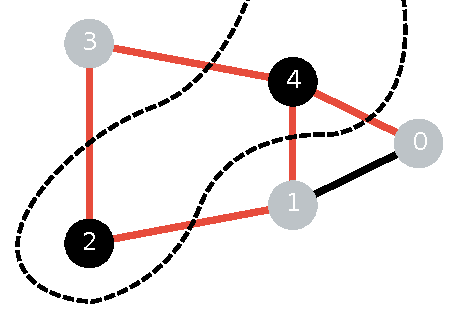
\includegraphics[width=0.4\linewidth]{figures/maxcut_5_graph_cut_example.pdf}
    \caption[Max-Cut example on a graph with five vertices and unit weights.]{
        Max-Cut example on a graph with five vertices and unit weights.
        The vertices are partitioned into two sets visualized as black and gray.
        The cut shown is a maximum cut with $L(z) = 5$, which can be thought of as the number of edges cut (shown in red).
    }
    \label{fig:maxcut-5-example}
\end{figure}

The \gls{qaoa} algorithm can be used for solving Max-Cut problems by assigning a vertex $j \in V$ to a qubit $\ket{q_j}$.
A qubit $\ket{q_j}$ is in state \ket{0} if a vertex $j$ is in partition $S$, and state \ket{1} if vertex $j$ is in partition $\bar{S}$.
To encode the objective function from \Cref{eqn:max-cut-objective}, note that the objective function can be rewritten as follows:
\begin{equation}
L(z) = \frac{1}{2} \sum_{(j, k) \in E} w_{j, k}(1 - z_jz_k),
\end{equation}
where $z_j \in \{-1, 1\}$ for $j \in V$.
This objective function can be represented by the following cost Hamiltonian:
\begin{equation} \label{eqn:problem-hamiltonian}
H_L = \frac{1}{2} \sum_{(j, k) \in E} w_{j, k}(I - Z^{(j)}Z^{(k)}).
\end{equation}
This gives the problem unitary
\begin{equation} \label{eqn:problem-unitary}
U(H_L, \gamma) = e^{-i\gamma H_L} = \prod_{(j, k) \in E} e^{-i\tfrac{\gamma}{2}w_{j, k}(I - Z^{(j)}Z^{(k)})},
\end{equation}
and the standard mixer unitary as defined in \Cref{sec:qaoa}:
\begin{equation} \label{eqn:mixer-unitary}
U(H_B, \beta) = e^{-i\beta H_B} = \prod_{j \in V} e^{-i\beta X^{(j)}}.
\end{equation}

\section{Implementation}
The \gls{qaoa} was implemented in Python using the Project Q~\cite{steiger2018projectq}, Quantum Inspire~\cite{quantuminspire}, and SciPy~\cite{scipy} frameworks to solve the Max-Cut problem on the graph from \Cref{fig:maxcut-4-graph}.
The optimal solutions for this graph are $z = 0101$ and $z = 1010$ with $L(z) = 4$.
\begin{figure}[ht]
    \centering
    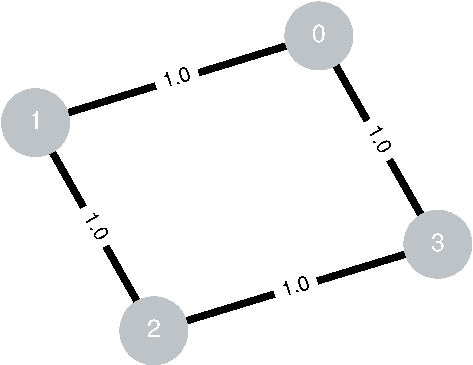
\includegraphics[width=0.4\linewidth]{figures/maxcut_4_graph.pdf}
    \caption{
        Undirected graph $G = (V, E)$ with $n = 4$ vertices $V = \{0, 1, 2, 3\}$ and 4 edges $E = \{(0,1), (0,3), (1,2), (2,3)\}$ with unit weight $w_{j, k} = w_{k, j} = 1$.
    }
    \label{fig:maxcut-4-graph}
\end{figure}
A $ZZ$ interaction $e^{-i\gamma/2(I - Z^{(j)}Z^{(k)})}$ from the problem unitary $U(H_L, \gamma)$ (\Cref{eqn:problem-unitary}) is implemented as follows:
\begin{figure}[H]
    \[
    \Qcircuit @C=1em @R=1em @!R {
        & \lstick{\ket{q_j}} & \ctrl{1} & \qw & \ctrl{1} & \qw \\
        & \lstick{\ket{q_k}} & \targ & \gate{Rz(-\gamma)} & \targ & \qw
    }
    \]
\end{figure}
\noindent
The $X$ interaction $e^{-i\beta X^{(j)}}$ from the mixer unitary $U(H_B, \beta)$ (\Cref{eqn:mixer-unitary}) is implemented as a $R_x$ gate:
\begin{figure}[H]
    \[
    \Qcircuit @C=1em @R=1em @!R {
        & \lstick{\ket{q_j}} & \gate{R_x(2\beta)} & \qw \\
    }
    \]
\end{figure}
\noindent
The complete quantum circuit for the \gls{qaoa} for Max-Cut on this graph is shown in \Cref{fig:qaoa-circuit}.

The quantum circuit is implemented using the ProjectQ quantum computing library.
To find the optimal parameters $\vec{\gamma}^*, \vec{\beta}^*$ the Nelder-Mead optimization algorithm~\cite{nelder1965simplex} provided by SciPy is used.
The relevant cost function is
\begin{equation}
C_p(\vec{\gamma}, \vec{\beta}) = \bra{\psi(\vec{\gamma}, \vec{\beta})}H_L\ket{\psi(\vec{\gamma}, \vec{\beta})},
\end{equation}
and we look to solve the optimization problem
\begin{equation}
\vec{\gamma}^*, \vec{\beta}^* = \argmax_{\vec{\gamma}, \vec{\beta}} C_p(\vec{\gamma}, \vec{\beta}).
\end{equation}
We then prepare the state $\ket{\psi(\vec{\gamma}^*, \vec{\beta}^*)}$ and measure multiple times in the computational basis to extract the solution, which is the bit string with the highest probability.

\begin{figure}
    \begin{adjustwidth}{-1cm}{-1cm}
    \[
    \Qcircuit @C=0.4em @R=0.8em @!R {
        & & & & & \lstick{\ket{q_0}} & \gate{H} & \qw & \ctrl{1} & \qw & \ctrl{1} & \qw & \ctrl{3} & \qw & \ctrl{3} & \qw & \qw & \qw & \qw & \qw & \qw & \qw & \qw & \qw & \gate{R_x(2\beta)} & \qw & \qw & \meter & \cw \\
        & & & & & \lstick{\ket{q_1}} & \gate{H} & \qw & \targ & \gate{R_z(-\gamma)} & \targ & \qw & \qw & \qw & \qw & \qw & \ctrl{1} & \qw & \ctrl{1} & \qw & \qw & \qw & \qw & \qw & \gate{R_x(2\beta)} & \qw & \qw & \meter & \cw \\
        & & & & & \lstick{\ket{q_2}} & \gate{H} & \qw & \qw & \qw & \qw & \qw & \qw & \qw & \qw & \qw & \targ & \gate{R_z(-\gamma)} & \targ & \qw & \ctrl{1} & \qw & \ctrl{1} & \qw & \gate{R_x(2\beta)} & \qw & \qw & \meter & \cw \\
        & & & & & \lstick{\ket{q_3}} & \gate{H} & \qw & \qw & \qw & \qw & \qw & \targ & \gate{R_z(-\gamma)} & \targ & \qw & \qw & \qw & \qw & \qw & \targ & \gate{R_z(-\gamma)} & \targ & \qw & \gate{R_x(2\beta)} \gategroup{1}{9}{4}{25}{1em}{--} & \qw & \qw & \meter & \cw \\
        & & & & & & & & & & & & & \hspace{5cm} p \mbox{ times}
    }
    \]
    \end{adjustwidth}
    \caption[Quantum circuit for the $p$-layer \gls{qaoa} on the graph from \Cref{fig:maxcut-4-graph}.]{
        Quantum circuit for the $p$-layer \gls{qaoa} on the graph from \Cref{fig:maxcut-4-graph}.
        Each vertex $j \in V$ is represented by qubit $\ket{q_j}$.
        The circuit starts by preparing an equal superposition state, after which the problem unitary $U(H_L, \gamma)$ and mixer unitary $U(H_B, \beta)$ are applied $p$ times.
        In general, the depth of the circuit is $p(3m + n)$, where $p$ is the number of layers, $m$ is the number of edges, and $n$ is the number of vertices. 
    }
    \label{fig:qaoa-circuit}
\end{figure}

\section{Results}
% TODO: results (simulation, hardware, different p)